%!TEX root = <main.tex>
\section{Experimental Evaluation}
We empirically validate if \system~ is able reduce the runtime taken for occlusion based deep CNN explainability workloads.
We then conduct controlled experiments to show the individual contribution of each optimization in \system~ for the overall system efficiency.

\vspace{2mm}
\noindent \textbf{Datasets.}
We use three real-world datasets: \textit{OCT}, \textit{Chest X-Ray}, and a sample from \textit{ImageNet}. \textit{OCT} has about 84,000 optical coherence tomography retinal images categorized into four categories: CNV, DME, DRUSEN, and NORMAL. CNV (choroidal neovascularization), DME (diabetic macular edema), and DRUSEN are three different varieties of Diabetic Retinopathy. NORMAL corresponds to healthy retinal images. \textit{Chest X-Ray} has about 6,000 X-ray images categorized into three categories: VIRAL, BACTERIAL, and NORMAL.
VIRAL and BACTERIAL categories correspond to two varieties of Pneumonia. NORMAL corresponds to chest X-Rays of healthy people. Both \textit{OCT} and \textit{Chest X-Ray} datasets are obtained from an original scientific study \cite{kermany2018identifying} which uses CNNs for predicting Diabetic Retinopathy and Pneumonia from radiological images. \textit{ImageNet} sample dataset contains 1,000 images corresponding to two hundred categories selected from the original thousand categorical dataset \cite{deng2009imagenet}.

\vspace{2mm}
\noindent \textbf{Workloads.}
We use three popular ImageNet-trained Deep CNNs: VGG16 \cite{vggnet}, ResNet18 \cite{resnet}, and Inception3 \cite{inception}, obtained from \cite{torchvisionmodels}.
They complement each other in terms of model size, computational cost, amount of theoretical redundancy that exist for occlusion experiments, and the level of architectural complexity of the CNN model.
For \textit{OCT} and \textit{Chest X-Ray} datasets the three CNN models are fine-tuned by retraining the final fully-connected layer with hyper-parameter tuning as per standard practice.
More details on the fine-tuning process are included in the Appendix.
Heat map for the predicted probabilities is generated using Python Matplotlib library's \texttt{imshow} method using the \texttt{jet\_r} color scheme.
For the heat map, the maximum threshold value is set to \texttt{min}$(1, 1.25 \times p)$ and minimum threshold value is set to $0.75 \times p$ where $p$ is predicted class probability for the unmodified image.
Original images were resized to the size required by the CNNs ($224\times224$ for VGG16 and ResNet18 and $299\times299$ for Inception3) and no additional pre-processing is done.
For GPU experiments a batch size of 128 and for CPU experiments a batch size 16 is used.
CPU experiments are executed with a thread parallelism of 8.
All of our datasets, fine-tuning, experiment, and system code will be made available on our project web page.

\vspace{2mm}
\noindent \textbf{Experimental Setup.}
We use a workstation which has 32 GB RAM, Intel i7-6700 @ 3.40GHz CPU, 1 TB Seagate ST1000DM010-2EP1, and Nvidia Titan X (Pascal) 12 GB memory GPU.
The system runs Ubuntu 16.04 operating system with PyTorch version of 0.4.0, CUDA version of 9.0, and cuDNN version of 7.1.2.
Each runtime reported is the average of three runs with 95\% confidence intervals shown.

\subsection{End-to-End Evaluation}

\begin{figure*}[t]
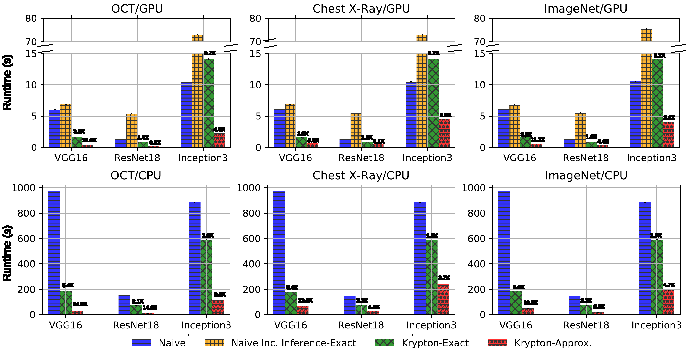
\includegraphics[width=\textwidth]{images/5_1_all_edited}
\caption{End-to-end efficiency achieved by \system~ over naive approaches.}
\label{fig:5_1_all_edited}
\end{figure*}

For the GPU based environment we compare two variations \system, \system-Exact which only applies the \textit{incremental inference} optimization and \system-Approximate which applies both \textit{incremental inference} and \textit{approximate inference} optimizations, against two baselines.
\textit{Naive} is the current dominant practice of performing full inference for multiple images with each corresponding to individual occlusion patch position in batched manner.
\textit{Naive Incremental Inference-Exact} is a pure PyTorch based implementation of Algorithm \ref{alg:incinference} which does not use any GPU optimized kernels for memory copying where as \system~ does.
For CPU based environments we only compare \system-Exact and \system-Approximate against \textit{Naive} as no customization is needed for the pure PyTorch based implementation.
For different datasets we set \textit{adaptive drill-down} system tuning parameters differently.
For \textit{OCT} images the region of interest is relative small and hence a $r_{drill-down}$ value of 0.1 and a target \texttt{speedup} of 5 is used.
For \textit{Chest X-Ray} images the region of interest can be large and hence a $r_{drill-down}$ value of 0.4 and a target \texttt{speedup} of 2 is used.
For \textit{ImageNet} experiments we use a $r_{drill-down}$ value of $0.25$ and a target \texttt{speedup} value of 3 which are also the \system~ default values.
For all experiments $\tau$ is configured using a separate tuning image dataset $(n=30)$ for a target SSIM of $0.9$.
Visual examples for each dataset is shown in Appendix.
Figure \ref{fig:5_1_all_edited} presents the final results.

We see that \system~ improves the efficiency of the occlusion based explainability workload across the board.
\system-Approximate for \textit{OCT} results in the highest speedup with VGG16 on both CPU and GPU environments (16X for CPU and 34.5X for GPU).
Speedups obtained by \system-Exact for all the datasets are same for all three CNN models.
However, with \system-Approximate they result in different speedup values.
This is because with \textit{approximate inference} each dataset uses different system configuration parameters.
\textit{OCT} which is configured with a low $r_{drill-down}$ of 0.1, high target \texttt{speedup} of 5, and a \textit{projective field threshold} value of 0.5 results in the highest speedup.
Speedup obtained by \system-Exact on GPU with Inception3 model (0.7X) is slightly lower than one.
However ResNet18 which has roughly the same theoretical speedup (see Figure \ref{fig:redundancy_ratio}) results in a higher speedup value (1.6X).
The reason for this is Inception3's internal architecture is more complex compared ResNet18 with more branches and depth-wise stacking operations.
Thus Inception3 requires more memory copying operations whose overheads are not captured by our theoretical speedup calculation.
Overall compared to GPU environment \system~ results in higher speedups on the CPU environment though the actual runtimes are much slower.
GPUs enable higher parallelism with thousands of processing cores compared to CPUs with several cores.
Hence computations are much cheaper on GPU.
Memory operations required by \system~ throttles the overall performance on GPU and hinders it from achieving higher speedups.
On CPU environment as computational cost dominates the overall runtime, the additional overhead introduced by the memory operations does not matter much.
Therefore on CPU \system~ achieves higher speedups which are closer to the theoretical speedup value.
Overall \system~ offers the best efficiency on these workloads.
This confirms the benefits of different optimizations performed by \system~ for improving the efficiency of the workload and thereby to reduce the computational and runtime costs.
Bringing down the runtimes also make occlusion experiments more amenable for interactive diagnosis of CNN predictions.


\subsection{Lesion Study}
We now present the results of controlled experiments that are conducted to identify the contribution of various optimizations discussed in Section \ref{sec:optimizer}.
The speedup values are calculated compared to the runtime taken by the current dominant practice of performing full inference for batches of modified images.

\begin{figure}[t]
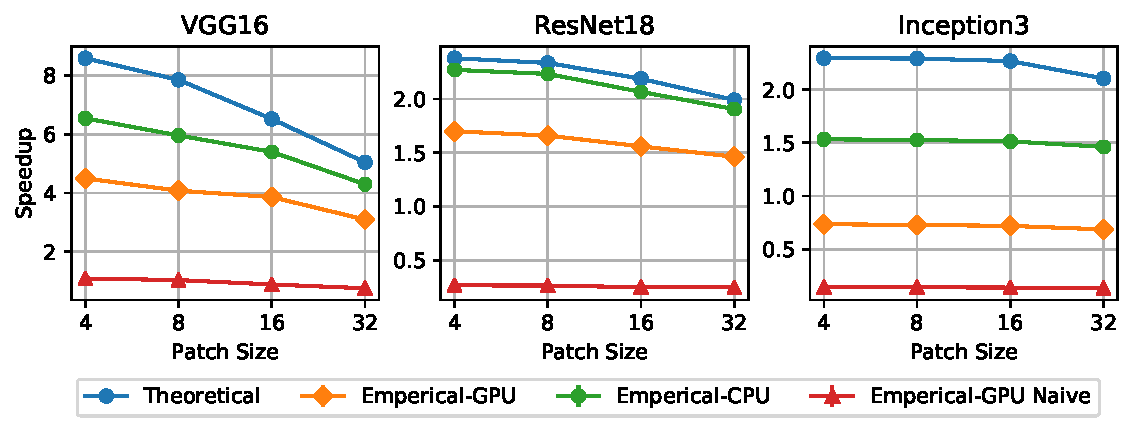
\includegraphics[width=\columnwidth]{images/5_2_1_edited}
\caption{Theoretical versus empirical speedup for \textit{incremental inference} (Occlusion patch stride $S=4$).}
\label{fig:5_2_1_edited}
\end{figure}

\vspace{2mm}
\noindent \textbf{Speedups from Incremental Inference.} We compare theoretical speedup and empirical speedups obtained by \textit{incremental inference} implementations for both CPU and GPU environments.
The patch sizes that we have selected cover the range of sizes used in most practical applications.
Occlusion patch stride is set to 4.
Figure \ref{fig:5_2_1_edited} shows the results.
Empirical-GPU Naive results in the worst performance for all three CNN models.
Empirical-GPU and Empirical-CPU implementations result in higher speedups with Empirical-CPU being closer to the theoretical speedup value.
As the occlusion patch size increases the speedups decrease.


\begin{figure}[t]
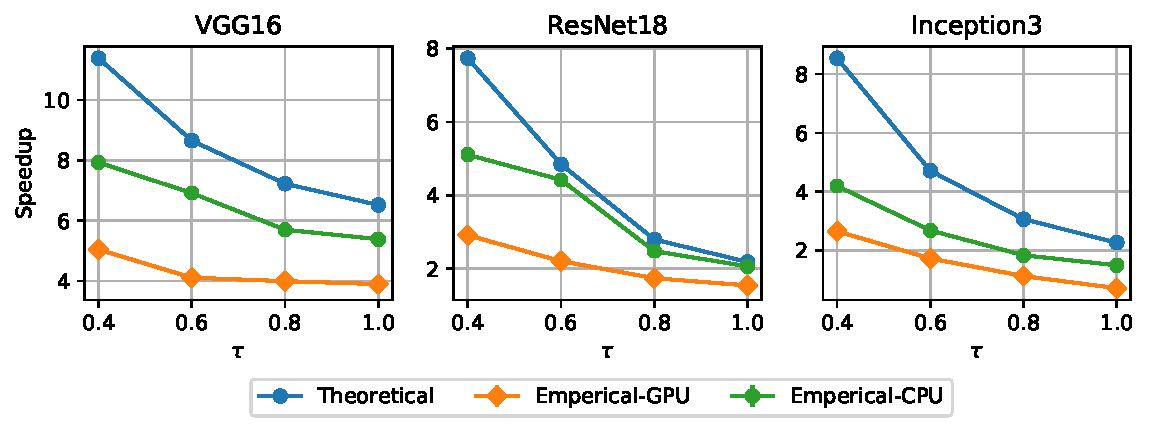
\includegraphics[width=\columnwidth]{images/5_2_2_edited}
\caption{Theoretical versus empirical speedup for \textit{incremental inference} with \textit{projective field thresholding} (Occlusion patch size = $16 \times 16$, stride $S=4$).}
\label{fig:5_2_2_edited}
\end{figure}

\vspace{2mm}
\noindent \textbf{Speedups from Projective Field Thresholding.} We vary \textit{projective field threshold} $\tau$ from 1.0 (no thresholding) to 0.4 and evaluate the speedups.
The occlusion patch size used is 16 and the stride is 4.
The results are shown in Figure \ref{fig:5_2_2_edited}.
Empirical-CPU and Empirical-GPU both results in higher speedups with Empirical-CPU being closer to the theoretical speedup value.
When $\tau$ decreases the speedups increase as the amount of computational savings increase.

\begin{figure}[t]
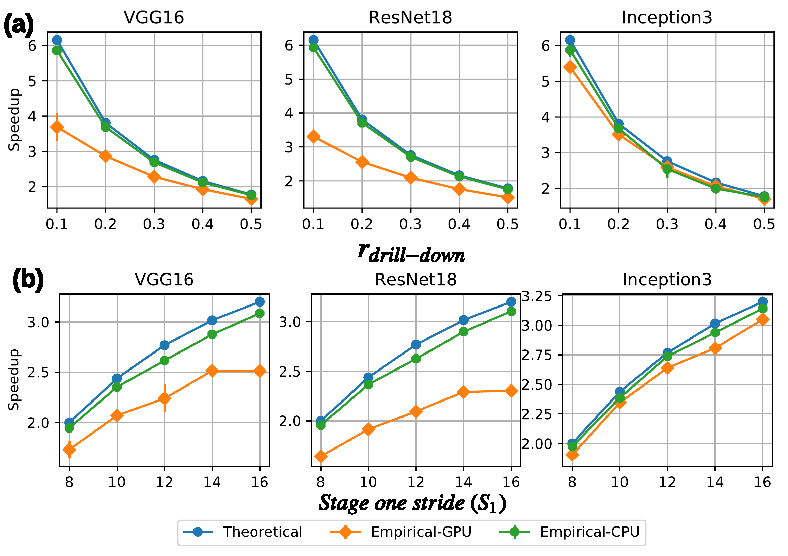
\includegraphics[width=\columnwidth]{images/5_2_3_edited}
\caption{Theoretical versus empirical speedup for \textit{adaptive drill-down} (Occlusion patch size = $16 \times 16$, stage two stride $S_2=4$, projective field threshold $\tau=1.0$. For (a) $S_1$=16 and for (b) $r_{drill\_down}$=0.25).}
\label{fig:5_2_3_edited}
\end{figure}

\vspace{2mm}
\noindent \textbf{Speedups from Adaptive Drill-Down.} Finally we evaluate the effect of \textit{adaptive drill-down} on overall \system~ efficiency.
The experiments are run on top of the \textit{incremental inference} approach with no \textit{projective field thresholding} ($\tau$=1.0).
$r_{drill-down}$ is varied between 0.1 to 0.5 fixing the stage one stride value $S_1$ to 16.
Occlusion patch size is set to 16 and the stage two stride $S_2$ is set to 4.
Figure \ref{fig:5_2_3_edited} (a) shows the results.
We also vary $S_1$ fixing $r_{drill-down}$ to 0.25.
Occlusion patch size and the $S_2$ are set same as in the previous case.
Figure \ref{fig:5_2_3_edited} (b) presents the results.
In both cases we see Empirical-GPU and Empirical-CPU achieve higher speedups with Empirical-CPU being very close to the theoretical speedup.
On the CPU environment, the relative cost of other overheads is much smaller than the CNN computational cost.
Hence on the CPU environment \system~ achieves near theoretical speedups for \textit{adaptive drill-down}.
Speedups decrease as we increase $r_{drill-down}$ and decrease $S_1$.

\vspace{2mm}
\noindent \textbf{Summary of Experimental Results.} Overall \system~ increases the efficiency of the occlusion based CNN explainability workload by up to 16X on GPU and 34.5X on CPU.
Speedup obtained by \textit{approximate inference} optimization (\system-Approximate) depends on the characteristics of the CNN model such as the effective growth of the projective field and the characteristics of the occlusion use case such as the relative size of the interesting regions on the image.
Furthermore \system~ results in higher speedups on CPU environment compared to GPU environment.
Increasing the occlusion patch size and $\tau$ decrease the speedup.
Increasing $r_{drill-down}$ and decreasing $S_1$ also decrease the speedup.

